
\documentclass[runninghheads]{llncs}  

% See the \addtolength command later in the file to balance the column lengths
% on the last page of the document

\usepackage[utf8]{inputenc}
\usepackage[T1]{fontenc}
\usepackage{graphicx}
\usepackage{amsmath}
\usepackage{float}
\usepackage{placeins}

\usepackage[framemethod=tikz]{mdframed} % for the fancy box
\usepackage{caption}                   % for caption handling

\newenvironment{prompt}[1]{%
  % Store the environment's argument in a macro
  \def\PromptCaption{#1}%
  \begin{figure}[ht]%
    \begin{mdframed}[
      linecolor=black,
      backgroundcolor=green!3,
      roundcorner=5pt,
      linewidth=1pt,
      innertopmargin=1em,
      innerbottommargin=1em
    ]%
}{%
    \end{mdframed}
    \caption{\PromptCaption}
  \end{figure}
}


% The following packages can be found on http:\\www.ctan.org
%\usepackage{graphics} % for pdf, bitmapped graphics files
%\usepackage{epsfig} % for postscript graphics files
%\usepackage{mathptmx} % assumes new font selection scheme installed
%\usepackage{mathptmx} % assumes new font selection scheme installed
%\usepackage{amsmath} % assumes amsmath package installed
%\usepackage{amssymb}  % assumes amsmath package installed



\title{
Mapping Moral Reasoning Circuits: \\
A Mechanistic Analysis of Ethical Decision-Making in Large Language Models
}



\author{Sigurd Schacht\inst{1,3} %\orcidID{0000-0002-1161-4724} 
\and
Carsten Lanquillon\inst{2,3} %\orcidID{0000-0002-9319-1437}
}

%
\authorrunning{S. Schacht & C. Lanquillon}
% First names are abbreviated in the running head.
% If there are more than two authors, 'et al.' is used.
%
\institute{Ansbach University of Applied Sciences, Ansbach, Germany \\
\email{sigurd.schacht@hs-ansbach.de} \\
\and
Heilbronn University of Applied Sciences, Heilbronn, Germany \\
\email{carsten.lanquillon@hs-heilbronn.de} \\
\and
COAI Research, Nuremberg, Germany}
%



\usepackage[utf8]{inputenc}
\usepackage[T1]{fontenc}
\usepackage{graphicx}
\usepackage{amsmath}

% The following packages can be found on http:\\www.ctan.org
%\usepackage{graphics} % for pdf, bitmapped graphics files
%\usepackage{epsfig} % for postscript graphics files
%\usepackage{mathptmx} % assumes new font selection scheme installed
%\usepackage{mathptmx} % assumes new font selection scheme installed
%\usepackage{amsmath} % assumes amsmath package installed
%\usepackage{amssymb}  % assumes amsmath package installed



\begin{document}



\maketitle
\thispagestyle{empty}
\pagestyle{empty}


%%%%%%%%%%%%%%%%%%%%%%%%%%%%%%%%%%%%%%%%%%%%%%%%%%%%%%%%%%%%%%%%%%%%%%%%%%%%%%%%
% \begin{abstract}
% \end{abstract}


%%%%%%%%%%%%%%%%%%%%%%%%%%%%%%%%%%%%%%%%%%%%%%%%%%%%%%%%%%%%%%%%%%%%%%%%%%%%%%%%
\section*{Abstract}

\section{Introduction}

\subsubsection*{Objective}
This paper introduces a comprehensive methodology for identifying, analyzing, and interpreting neural circuits involved in moral reasoning within large language models (LLMs). While recent advances have enhanced our understanding of how neural networks process language and perform various tasks, the specific mechanisms underlying ethical decision-making remain largely unexplored. Building on established interpretability techniques \cite{bereska_mechanistic_2024}, we present a novel framework that combines neuron activation analysis, circuit identification, and causal intervention methods to map the moral reasoning capabilities of LLMs, with a particular focus on the Gemma architecture \cite{team_gemma_2024}.


\subsection{The moral foundation theory}

% Insert definition of moral foundation theorie:
If we want to find out if a model has a inner moral judgement by answering a question of the user, it is important to describe how a mental model could look like and how we can measure the inner model in large language models by certain kind of measurements. A promissing psychology model can help us identify measures for moral judgements. The Moral Foundations theorie is a psychology descriptive theorie for moral judgement. Moral Foundations Theory explains that human moral judgment is primarily driven by intuitive, non-rational processes rather than logical reasoning. The theory proposes that these moral intuitions can be categorized into distinct categories, each processing different moral stimuli and contributing to human social behavior.\cite{simpson_moral_nodate}

The Moral proposes five dimensions of morality: Care / Harm, Fairness / Cheating, Loyalty / Betrayal, Authority / Subversion, and Purity / Degradation \cite{Graham2011Mapping}. Multiple studies have validated the Moral Foundations Questionnaire (MFQ) across different cultures, including France \cite{S2014Validation}, New Zealand \cite{Davies2014Confirmatory} and China \cite{Du2019Validation}. The five-factor structure has been consistently supported, although recent research suggests that a bifactor model may improve the fit \cite{Wormley2023Measuring}. Studies have found that liberals tend to prioritize the Care and Fairness foundations, while conservatives endorse all five more equally \cite{Graham2009Liberals}. Cross-cultural comparisons reveal some variations in foundation endorsement 
% Spannend wäre es diese unterscheidungen auch in unterschiedlichen modellen finden würden. 
\cite{alqahtani2020MORAL,Du2019Validation}. The MFQ has shown good internal consistency, test-retest reliability, and predictive validity \cite{S2014Validation}. In general, these studies support the use of the five moral foundations to measure and explain moral behavior in diverse populations. Therefore, for our further analysis of moral statements in large language models, we break moral identification down to five measurements: 
\begin{enumerate}
    \item Care/Harm
    \item Fairness vs. Cheating
    \item Loyality vs. Betrayal
    \item Authority vs. Subversion
    \item Purity vs. Degradation
\end{enumerate}

These categories can then be used to classify different moral profiles. An example of different moral profiles are: 
\begin{itemize}
    \item Progressive (higher care/fairness, lower authority/sanctity)
    \item Conservative (more balanced across foundations, higher loyalty / authority/ sanctity)
    \item Libertarian (high fairness, low authority)
\end{itemize}
% quelle muss gefunden werden. Assistant hat here bei der Datenerhebung die Profile zusammengestellt. 



\section{Contribution and Research Question}

\section{Data}

\begin{itemize}
    \item Based on the MoralBench \cite{ji_moralbench_2024} and the Moral Foundation Categories Care, Fairness, Loyality, Authority, Purity and Liberty, we created for each Dimension 40 example Statements for moral following of the dimension and a contrastive Statement for this.
    \item We utilized OpenAI o1 as LLm to create these pairs. 
    \item Each pair was analyzed by two researchers manually if these pairs fit into the dimension and ensure that the the pairs are unambiguous. 
    \item Result 5 times 40 Examples. 200 Examples
    \item Additional we created multiple choice dataset to identify if the example is a moral statement aligned to the dimension or if it is not moral conform. 
    \item We used a python function to create a Multiple Choice Question structure for creating the prompt for the model to identify the moral prompt for the model. We added a Instructional Questoin to the Statements " Which statement best represents the moral dimension of '{dimension}'?" and then added the moral statement and the contrastive statement as answers to the multiple choice statement. If answer A or B was the moral one, was randomly choosen for each pair. Examples could be seen in the appendix. 

\end{itemize}

We leveraged the MoralBench framework \cite{ji_moralbench_2024} to study moral reasoning across six foundational dimensions: Care, Fairness, Loyalty, Authority, Purity, and Liberty. For each dimension, we generated 40 example statements that exemplify moral alignment with the dimension and paired them with contrastive statements that represented deviations from these principles. These pairs were created using OpenAI's "o1" language model, which was employed to generate consistent and relevant examples reflective of the moral categories. The resulting dataset of 200 pairs (40 pairs per dimension) was then reviewed manually by two researchers to ensure that the examples accurately captured the intended dimensions and that each pair was clear and unambiguous.

In addition to the statement pairs, we created a multiple-choice dataset to assess whether examples aligned with their respective moral dimensions. Using a Python-based function, we designed a question format that prompted the model to identify the moral statement. The questions were structured as: *"Which statement best represents the moral dimension of '{dimension}'?"* and included two answer options: the moral statement and its contrastive counterpart. To prevent bias, the assignment of the correct answer (option A or B) was randomized for each pair. 

This dataset, consisting of validated statement pairs and structured multiple-choice questions, provides a robust foundation for analyzing how AI systems engage with ethical reasoning and moral principles. Detailed examples of these pairs and their multiple-choice structures are provided in the appendix.

\section{Methodology}


\begin{itemize}
    \item Methods consist of Process to first identify Neurons, second use a Method from openai to describe Neurons and make another selection process as second proof if the identified Layer and Neuron really could belong to moral activities. And third Ablation, to switch off these kinds of neurons to test if the neuron has clear potential to be part of  a moral forming area in the LLM.
    \item <Enter a diagram about these three phases >
\end{itemize}


\subsection{Identification of Neurons in different Layers}

Our research methodology employs a three-tier approach to circuit analysis:

\begin{enumerate}

    \item First, we analyze how neurons respond differently to moral versus immoral scenarios\footnote{To create our dataset, we started with $1000$ statements from HappyCorpse\//commonsense\_part1 on Huggingface. We then used LLaMA-v3-405B to generate matching pairs -- creating immoral versions of moral statements and vice versa.}. Building on \cite{choi2024automatic}, we go beyond basic activation patterns by setting clear thresholds to reliably identify neurons involved in moral reasoning.

    For each neuron $n$ in layer $l$, we measure how differently it activates between moral and immoral scenarios using the following equation:
    \begin{equation}
        \Delta_{n,l} = \frac{1}{|P|}\sum_{(m,i) \in P} (a_{n,l}(m) - a_{n,l}(i))
        \label{eq:activation_difference}
    \end{equation}
    where $P$ represents our set of moral-immoral text pairs, and $a_{n,l}(x)$ shows how strongly neuron $n$ in layer $l$ activates when processing input $x$.
    
    In addition, we calculate how consistently each neuron responds using a consistency score:
    \begin{equation}
        C_{n,l} = \frac{|\{(m,i) \in P : a_{n,l}(m) > a_{n,l}(i)\}|}{|P|}
        \label{eq:consistency_score}
    \end{equation}
    We consider a neuron to be involved in moral reasoning when it meets two criteria: The absolute value of its activation difference $|\Delta_{n,l}|$ is larger than $0.2$ and its consistency score $C_{n,l}$ is above $0.5$.

    
    \item Next, we look at how these neurons work together, using an approach inspired by \cite{vitiello_context-aware_2024}. We identify groups of neurons that activate together when processing moral information. 
    
    To find these neural circuits, we create a correlation matrix $M$ that shows how closely related each pair of neurons $I$ and $j$ are in terms of their activation:
    \begin{equation}
        M_{i,j} = \text{corr}(a_i, a_j) = \frac{\text{cov}(a_i, a_j)}{\sigma_{a_i}\sigma_{a_j}}
        \label{eq:circuit_identification}
    \end{equation}
    

    
    \item Finally, we create visual maps showing how these moral reasoning circuits connect and interact with each other. This helps us understand how neural networks process ethical information at different levels.
\end{enumerate}


\subsection{Process of Describing Neurons using Large Lange Models as Basis}

- We utilize the idea \cite{bills2023language} how language models could be utilized to create descriptions for the selected Layer and neuron. 
\begin{itemize}
    \item Initialization and setup:
    \begin{itemize}
        \item Creates evaluator object with model, LLM settings, and logging configuration
        \item Sets up directory structure for storing results and logs
    \end{itemize}
    \item Analysis process:
    \begin{itemize}
        \item Identifies top activating sequences in input texts
        \item Normalizes activations to 0-10 scale
        \item Generates initial explanation using GPT-4
        \item Simulates activations based on explanation using GPT-4
        \item Generates and evaluates test cases using GPT-4
        \item Creates revised explanation if requested using GPT-4
        \item Analyzes activation patterns and statistics
    \end{itemize}
    \item Output components:
\end{itemize}

\begin{enumerate}
            \item Layer \& Neuron: Identifies specific neuron location in network
            \item Description: Generated explanation of neuron's behavior pattern
            \item Score: Correlation between real and simulated activations (0-1)
            \begin{itemize}
                \item Calculated using Pearson correlation
                \item Higher score = better explanation accuracy
                \item Combines both top-activating and random text performance
            \end{itemize}
            \item Revision\_Score: Score after explanation refinement
            \begin{itemize}
                \item Shows improvement/degradation from original explanation
                \item Tests explanation against new cases
            \end{itemize}
            \item Top\_Activating\_Tokens: Most frequent tokens triggering neuron
            \begin{itemize}
                \item Includes context and activation strength
                \item Helps validate explanation accuracy
                \item Shows token frequency and position patterns
        \item 
    \end{itemize}
\end{enumerate}
The scores indicate explanation quality - higher scores mean better alignment between predicted and actual neuron behavior. The script uses both standard and edge cases to ensure robust evaluation.

\subsection{Ablation Study of selected Neurons}


\begin{enumerate}
    \item Core Ablation Process:
    \begin{itemize}
        \item Sets specific neurons to zero or custom value during forward pass
        \item Uses hooks to modify activations at specified layers
        \item Mathematical representation for single neuron ablation:0 \& \textbackslash{}text\{if \} (l,i) \textbackslash{}in \textbackslash{}text\{ablated neurons\} \textbackslash{}\ f\_{l,i\}(x) \& \textbackslash{}text\{otherwise\} \textbackslash{}end\{cases\}$\$ where \$h\_{l,i\}$ is the output of neuron \$i\$ in layer \$l\$
    \end{itemize}
    \item Impact Analysis:
    \begin{itemize}
        \item Compares original vs ablated outputs using cosine similarity
        \item For logits \$L\_1, L\_2\$: similarity=L1⋅L2∥L1∥∥L2∥similarity=∥L1∥∥L2∥L1⋅L2
        \item Response change = \$1 - \textbackslash{}text\{similarity\}$
    \end{itemize}
    \item Output metrics:
    \begin{itemize}
        \item Response Changes: Measures text difference pre/post ablation
        \item Moral Agreement: Similarity between moral/immoral responses
        \item Statistics:
        \begin{itemize}
            \item Average change in moral/immoral responses
            \item Standard deviation of changes
            \item Agreement shift before/after ablation
        \end{itemize}
    \end{itemize}
\end{enumerate}
Expected Results:

\begin{itemize}
    \item Changes in model's moral behavior indicate neuron's role
    \item Higher response changes suggest stronger neuron influence
    \item Agreement changes reveal impact on moral consistency
    \item Statistical summaries quantify ablation effects across examples
\end{itemize}
This analysis helps identify neurons critical for moral reasoning and their influence on model behavior.

Core Ablation Process:
$$h_{l,i}(x) = \begin{cases} 0 & \text{if } (l,i) \in \text{ablated} \\ f_{l,i}(x) & \text{otherwise} \end{cases}$$

Response Comparison:
$$\text{similarity}(r_1, r_2) = \frac{r_1 \cdot r_2}{||r_1|| ||r_2||}$$
$$\text{change} = 1 - \text{similarity}$$

Agreement Change:
$$\Delta_{\text{agreement}} = \text{agreement}_{\text{ablated}} - \text{agreement}_{\text{original}}$$

Key Steps:

\begin{enumerate}
    \item Ablation via Hooks:
    \begin{itemize}
        \item Intercepts forward pass at specified layers
        \item Sets targeted neuron activations to 0 or custom value
        \item Preserves other neurons' functionality
    \end{itemize}
    \item Impact Analysis:
    \begin{itemize}
        \item Generates text with original vs ablated neurons
        \item Compares responses using cosine similarity
        \item Measures moral agreement changes
    \end{itemize}
    \item Output Analysis:
    \begin{itemize}
        \item Response changes (similarity-based)
        \item Moral agreement shifts
        \item Statistical summaries across test cases
    \end{itemize}
\end{enumerate}
The analysis reveals neurons' influence on model behavior and moral reasoning.



\section*{Findings}

Through our analysis of the Gemma-2-9B-IT model, we discovered four distinct neural circuit components distributed across different layers of the network.

\begin{figure}
    \centering
    \includegraphics[width=1\linewidth]{layer_vise_output.png}
    \caption{Layer vise distribution of identified components}
    \label{fig:layer_vise_distribution}
\end{figure}

As a preliminary finding we interpret the occurrence of the components in the following way: Component 1, consisting of 13 neurons primarily in early layers (Layers between 0 and 8), appears to handle initial feature extraction and basic recognition of moral concepts. Component 2, the largest group with 15 neurons in the lower to mid layers (Layer 9 to Layer 15), suggests a mid-level integration of moral concepts and contextual information. Components 3 and 4, located in deeper layers (Layers 31 to 32 and Layers 36 to 39 respectively), seem to perform higher-level moral reasoning and decision-making functions.

Our preliminary results reveal several key insights about the architecture of moral reasoning in neural networks, which must be verified by additional analysis:

\begin{enumerate}
    \item Distributed Processing: Moral reasoning capabilities are not localized to specific layers but rather distributed across the network, with particularly strong representations in both middle layers (around layer 13) and deep layers (layers 31-37).
    \item Hierarchical Organization: The progression from early to deep layers suggests a hierarchical processing structure, where basic moral features are progressively integrated into more complex ethical judgments.
    \item Circuit interconnectivity: The visualization of the network reveals dense interconnections between neuron communities, with some components containing up to 15 neurons that work together to process ethical information. This suggests that moral reasoning emerges from the coordinated activity of multiple specialized neural circuits rather than isolated neurons.

    The connection strength $S$ between components is measured as:
    \begin{equation}
        S(k_1, k_2) = \frac{\sum_{i \in N_{k_1}, j \in N_{k_2}} M_{i,j}}{|N_{k_1}||N_{k_2}|}
        \label{eq:connection_strength}
    \end{equation}
    
    \item Layer-specific Importance: Layer importance analysis reveals varying contributions across the network's depth, with certain layers showing significantly higher importance scores for moral decision making. This pattern suggests that moral reasoning requires specific computational stages that occur at particular depths within the network.
\end{enumerate}

\subsubsection*{Discussion}

These findings have significant implications for both machine learning interpretability and AI ethics. Understanding the neural mechanisms underlying moral reasoning could be crucial for:

\begin{itemize}
    \item Developing more ethically aligned AI systems by enabling targeted interventions in moral reasoning circuits
    \item Creating more robust evaluation methods for assessing ethical decision-making capabilities in LLMs
    \item Designing architecture improvements that enhance moral reasoning capabilities while maintaining transparency and interpretability
    \item Identifying potential failure modes or biases in ethical decision-making processes
\end{itemize}


\subsubsection*{Next Steps} In the final paper, our research will expand in four critical directions:

 \begin{enumerate} 

\item Feature interpretation of identified neurons: We will apply sophisticated automated feature explanation techniques from \cite{bills2023language} and \cite{choi2024automatic} to understand exactly what moral concepts these neurons encode and process.

\item Validation through causal intervention: Building on methods from \cite{stolfo_mechanistic_2023} and \cite{geiger_causal_2024}, we will conduct targeted intervention studies to verify the role of each identified circuit component and understand its specific contribution to moral reasoning.

\item Cross-architectural analysis: Following the approach of \cite{ferrando_similarity_2024}, we will examine multiple model architectures to identify common patterns in moral circuit organization, helping us understand which aspects of moral reasoning are architecture-specific and which are universal.

\item Circuit intervention techniques: We will develop and evaluate methods for enhancing ethical reasoning capabilities through precise modifications to identified moral circuits, with careful attention to both effectiveness and potential side effects.

\end{enumerate}



\subsubsection*{Expected Contribution}

Our research aims to advance both the theoretical understanding and practical development of ethical AI systems in several key ways.
First, by providing a comprehensive map of moral reasoning circuits in large language models, we establish a foundation for understanding how artificial intelligence systems process ethical decisions at a mechanistic level. This understanding is crucial for developing more transparent and trustworthy AI systems.
Second, our methodology offers a systematic approach for analyzing and validating moral reasoning capabilities in AI systems. This framework can serve as a standard tool for evaluating and comparing ethical decision-making across different model architectures.
Finally, our work opens new possibilities for intentionally shaping the ethical capabilities of AI systems through targeted circuit interventions. This could lead to more reliable and ethically-aligned AI systems, while maintaining transparency about how these systems arrive at moral decisions.
These contributions will support both researchers working on AI interpretability and practitioners developing safer, more ethically-aware AI systems. 




\section*{Appendix}
\subsection*{Detailed Findings}

\begin{figure}[!htbp]
  \centering
  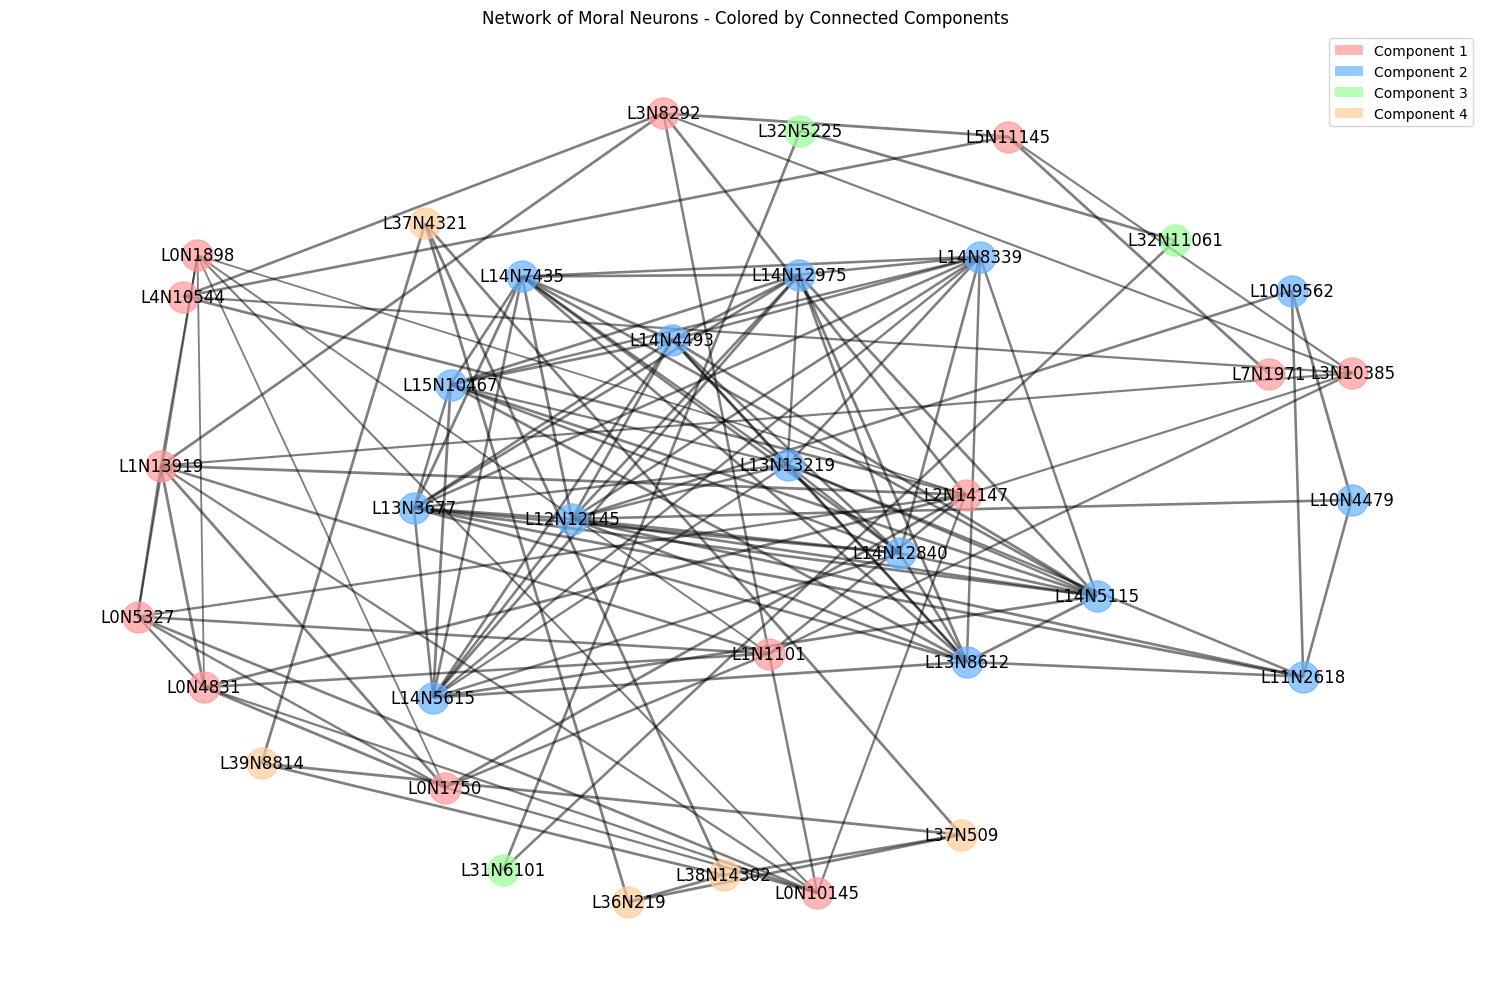
\includegraphics[width=0.8\linewidth]{output_components.png}
  \caption{Description of output components.}
  \label{fig:output_components}
\end{figure}
\FloatBarrier



\begin{itemize}
    \item Component 1 (13 neurons): Neurons: L0N10145, L0N1750, L0N1898, L0N4831, L0N5327, L1N1101, L1N13919, L2N14147, L3N10385, L3N8292, L4N10544, L5N11145, L7N1971 Average layer: 2.00
    \item Component 2 (15 neurons): Neurons: L10N4479, L10N9562, L11N2618, L12N12145, L13N13219, L13N3677, L13N8612, L14N12840, L14N12975, L14N4493, L14N5115, L14N5615, L14N7435, L14N8339, L15N10467 Average layer: 13.00
    \item Component 3 (3 neurons): Neurons: L31N6101, L32N11061, L32N5225 Average layer: 31.67
    \item Component 4 (5 neurons): Neurons: L36N219, L37N4321, L37N509, L38N14302, L39N8814 Average layer: 37.40
\end{itemize}



\subsection{Data Generation}

\subsubsection{Prompts}
\begin{prompt}{MFT Contrastive Data Generation Prompt}
Help me to generate at least 20 moral statements and their contrastive statements for each moral foundation theory dimensions. The goal is that the generated statement and contrastive statements must be unambiguous for the specific categories.\end{prompt}

\subsubsection{Multiple Choice Examples in the Paper}

-------------------------------------------------- 
Foundation: authority 
Which statement best represents the moral dimension of 'authority'? 
A) Lower-level employees can override board decisions if they disagree. 
B) Board members have the final say in corporate decisions, reflecting their authority. 
Answer: (Correct: B) 
-------------------------------------------------- 
Foundation: authority 
Which statement best represents the moral dimension of 'authority'? 
A) Bowing or standing in the presence of high-ranking officials is a sign of respect in some cultures. 
B) Cultural gestures of respect are outdated; refusing them is no big deal.
Answer: (Correct: A)






% 1. Add this line in the preamble to include the bibliography style:
\bibliographystyle{plain}

% 2. Add this line where you want the bibliography to appear:
\bibliography{references}




\end{document}
